\subsection{Cathode to anode ratio spread}

The cathode to anode ratio values found in this investigation were used to attempt to determine depth of interaction and to perform energy correction. DOI values derived from CAR were clustered between 0 and 1, and scatter plots showed features corresponding to peaks (which have been observed in other investigations, cite{Knoll,He}). A small fraction (less than 5 percent) of all C-A scatter points were outside the valid value range, indicating either spurious coincidence or poor charge collection. 

Attempts to correct spectra using CAR and 

[SECTION ON TIMING DOI DETERMINATION]


\begin{figure}[h!]
\begin{center}
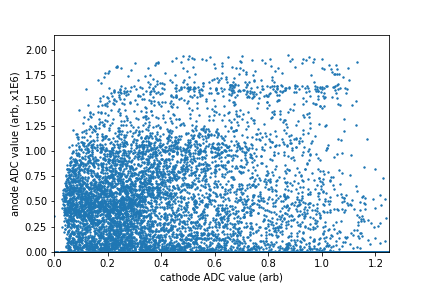
\includegraphics[scale=0.5]{scatter.png}
\caption{This scatterplot shows coincident events as points in cathode-anode space. The distribution of these points shows a strong clustering below cathode values of 4E6 and anode values of 1.2E7. Manually plotting these events shows that these are primarily low-energy events clustered near the anode layer. There is an additional near-horizontal band near an anode value of 1.55E7, which are primarily photopeak events. }
\label{rt}
\end{center}
\end{figure}
\clearpage



\begin{figure}[h!]
\begin{center}
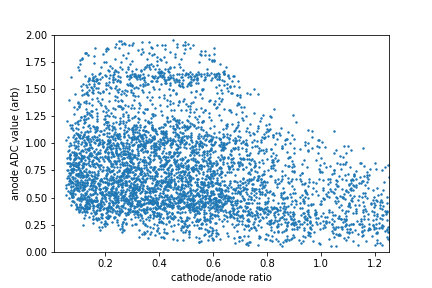
\includegraphics[scale=0.5]{scatter_CAR.png}
\caption{This scatter plot of the anode value versus the cathode/anode ratio demonstrates the banding structure associated with the photopeak clearly near an anode value of 1.55E6. The events with CAR values >1 are mostly spurious coincidence, and will increase in number with larger window settings. Strong clustering is evident at CAR values below .75.}
\label{Ori}
\end{center}
\end{figure}



\begin{figure}[h!]
\begin{center}
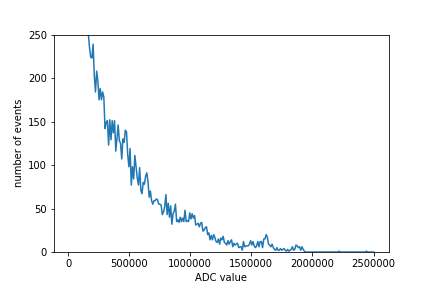
\includegraphics[scale=0.5]{all_anode_pulses.png}
\caption{The energy spectrum associated with all anode events shows extreme low-energy tailing and what appear to be spurious peaks. This spectrum resulted from events occuring at all pixels, and does not exclude anode events with no corresponding cathode pulse. }
\label{400}
\end{center}
\end{figure}


\begin{figure}[h!]
\begin{center}
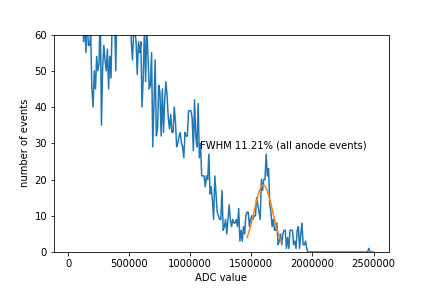
\includegraphics[scale=0.5]{CAR_all.png}
\caption{The energy spectrum associated with all anode events with coincidence shows greatly improved peak resolution, though the number of events has been reduced by an order of magnitude. The fitted FWHM is poor in comparison to most commercial CZT systems, which may be due to depth effects, charge trapping or noise problems.}
\label{400}
\end{center}
\end{figure}


\begin{figure}[h!]
\begin{center}
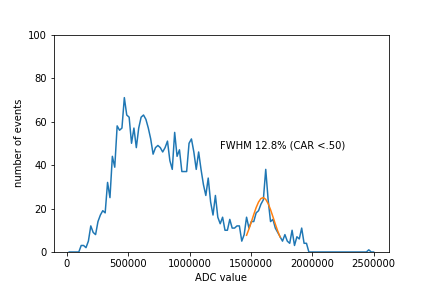
\includegraphics[scale=0.5]{CAR1_all.png}
\caption{Further filtering the coincident anode events by CAR drastically reduces the low-energy background and improves peak FWHM. The fitted FWHM remains poor in comparison to most commercial CZT systems, which may be due to depth effects, charge trapping or noise problems.}
\label{400}
\end{center}
\end{figure}

\begin{figure}[h!]
\begin{center}
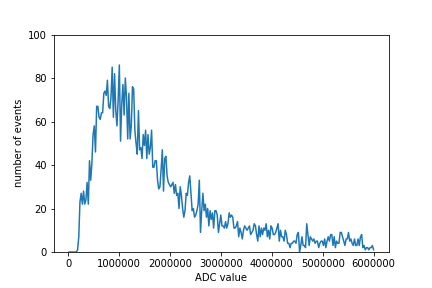
\includegraphics[scale=0.5]{corr_anode_pulses.png}mu
\caption{Attempts to correct the "all coincident pulses" anode data using the Hecht relation was unsuccessful, as is shown in this plot. This may be due to improper mu-tau data or improper correction factor application. This is a focus of future of work.}
\label{400}
\end{center}
\end{figure}

\begin{figure}[h!]
\begin{center}
\includegraphics[scale=0.5]{anodes_px.png}
\caption{Plotting coincident events by anode number demonstrates that pixels 7-8 have significantly different gain and resolution properties. Pixel 1 shows outstanding resolution in comparison to 2-6.}
\label{400}
\end{center}
\end{figure}

\begin{figure}[h!]
\begin{center}
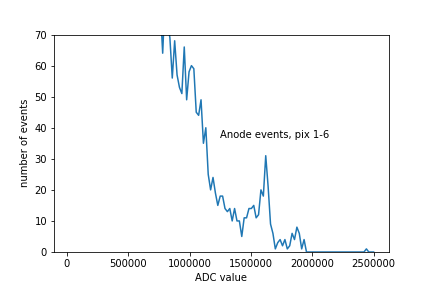
\includegraphics[scale=0.5]{anodes_1_6.png}
\caption{Re-plotting coincident events while excluding anodes 7-8 shows a significant improvement in resolution. This result was durable when tested at different bias voltages and data sets. This will be investigated in the near future.}
\label{400}
\end{center}
\end{figure}




\end{figure}


